

\pgfplotstableread[col sep=comma]{fw_thres_test_bio-dmela/fw_thresh_bio-dmela.csv}\fwtbm
\pgfplotstableread[col sep=comma]{fw_thres_test_bio-dmela/fw_thres_bd_times.csv}\fwtbmt
\begin{figure}[H]
    \centering
    %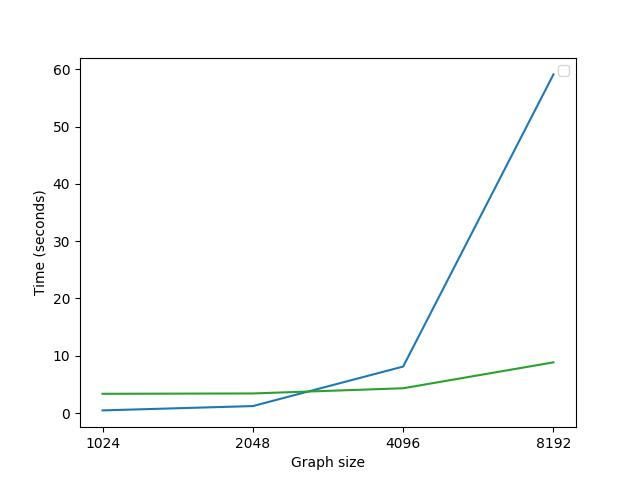
\includegraphics[width=\textwidth]{figures/sparse_vs_normal_gradient_time.jpg}
    \begin{tikzpicture}
        \begin{axis}[
                width=\linewidth*0.5,
                xlabel={Noise},
                ylabel={Accuraccy},
                x dir=reverse,
                legend pos=south west,
                xtick=data,
                xticklabels={$0.0$, $0.1$, $0.2$, $0.3$, $0.4$, $0.5$},
                %yticklabel={\pgfmathprintnumber[fixed,precision=2]{\tick}},
                legend style={at={(0.5,-0.20)}, anchor=north, legend columns=3,},
                ymajorgrids=true,
                xmajorgrids=true,
            ]
            \pgfplotsforeachungrouped \i in {1,2,3,4,5,6} {
                    \addplot table[x index=0, y expr=\thisrowno{\i}]
                        {\fwtbm};
                }
            \legend{$\gamma = 0.00$, $\gamma = 0.05$, $\gamma = 0.10$, $\gamma = 0.20$, $\gamma = 0.50$, $\gamma = 1.00$}
        \end{axis}
    \end{tikzpicture}
    \caption{Accuracy of different levels of $\gamma$. \textsc{cuGAL} with Sinkhorn-Knopp-mix \ref{alg:sinkhorn_mix} on bio-dmela}
    \label{fig:FW_accu}
\end{figure}
\hfill
\begin{figure}[H]
    \begin{tikzpicture}
        \begin{semilogyaxis}[
                width=\linewidth,
                ybar stacked,
                log origin=infty,
                ylabel={Time $(s)$},
                xlabel={Noise},
                bar width=6pt,
                legend pos=south west,
                xtick=\empty,%{3.5, 10.5, 17.5, 24.5, 31.5, 38.5},
                %xticklabels={0, 5, 10, 15, 20, 25},
                %x tick label style={\empty}
                %extra x tick style={xshift=,},
                legend style={at={(0.5,-0.1)}, anchor=north, legend columns=-1},
                %yticklabel={\pgfmathprintnumber[fixed,precision=2]{\tick}},
                ymajorgrids=true,
                xmajorgrids=true,
            ]
            \pgfplotsforeachungrouped \i in {0,1,2,3} {
                    \addplot table[x expr=\coordindex, y index=\i]
                        {\fwtbmt};
                }

            %\legend{$ \displaystyle { \text{Sinkhorn-} \atop \text{Knopp} }$, $ \displaystyle { \text{Feature} \atop \text{Extraction} }$, Gradient, Hungarian};
            \legend{Sinkhorn-Knopp-mix \ref{alg:sinkhorn_mix}, Feature Extraction, Gradient \ref{alg:cugal-calculate-gradient}, Hungarian};
            \coordinate (brace1start) at (axis cs:0,0);
            \coordinate (brace1end) at (axis cs:7.5,0);
            \coordinate (brace2start) at (axis cs:4.5,10);
            \coordinate (brace2end) at (axis cs:8.5,10);
            \coordinate (brace3start) at (axis cs:8.5,10);
            \coordinate (brace3end) at (axis cs:12.5,10);
            \coordinate (brace4start) at (axis cs:12.5,10);
            \coordinate (brace4end) at (axis cs:16.5,10);
        \end{semilogyaxis}
        % Adding the braces
        \draw [decorate,decoration={brace,amplitude=10pt,mirror,raise=4ex}]
        (brace1start) -- (brace1end) node[midway,yshift=-3em]{0 noise};
        \draw [decorate,decoration={brace,amplitude=10pt,mirror,raise=4ex}]
        (brace2start) -- (brace2end) node[midway,yshift=-3em]{5 noise};
        \draw [decorate,decoration={brace,amplitude=10pt,mirror,raise=4ex}]
        (brace3start) -- (brace3end) node[midway,yshift=-3em]{10 noise};
        \draw [decorate,decoration={brace,amplitude=10pt,mirror,raise=4ex}]
        (brace4start) -- (brace4end) node[midway,yshift=-3em]{0.3 noise};

    \end{tikzpicture}
    \caption{Speed of different levels of $\gamma$. There are six levels of increasing noise, each tested with six increasing $\gamma$ thresholds.}
    \label{fig:FW_speed}
\end{figure}